\documentclass[a4paper]{article}

%================================================================================================================================
%
% Packages
%
%================================================================================================================================

\usepackage[T1]{fontenc} 	% pour caractères accentués
\usepackage[utf8]{inputenc}  % encodage utf8
\usepackage[french]{babel}	% langue : français
\usepackage{fourier}			% caractères plus lisibles
\usepackage[dvipsnames]{xcolor} % couleurs
\usepackage{fancyhdr}		% réglage header footer
\usepackage{needspace}		% empêcher sauts de page mal placés
\usepackage{graphicx}		% pour inclure des graphiques
\usepackage{enumitem,cprotect}		% personnalise les listes d'items (nécessaire pour ol, al ...)
\usepackage{hyperref}		% Liens hypertexte
\usepackage{pstricks,pst-all,pst-node,pstricks-add,pst-math,pst-plot,pst-tree,pst-eucl} % pstricks
\usepackage[a4paper,includeheadfoot,top=2cm,left=3cm, bottom=2cm,right=3cm]{geometry} % marges etc.
\usepackage{comment}			% commentaires multilignes
\usepackage{amsmath,environ} % maths (matrices, etc.)
\usepackage{amssymb,makeidx}
\usepackage{bm}				% bold maths
\usepackage{tabularx}		% tableaux
\usepackage{colortbl}		% tableaux en couleur
\usepackage{fontawesome}		% Fontawesome
\usepackage{environ}			% environment with command
\usepackage{fp}				% calculs pour ps-tricks
\usepackage{multido}			% pour ps tricks
\usepackage[np]{numprint}	% formattage nombre
\usepackage{tikz,tkz-tab} 			% package principal TikZ
\usepackage{pgfplots}   % axes
\usepackage{mathrsfs}    % cursives
\usepackage{calc}			% calcul taille boites
\usepackage[scaled=0.875]{helvet} % font sans serif
\usepackage{svg} % svg
\usepackage{scrextend} % local margin
\usepackage{scratch} %scratch
\usepackage{multicol} % colonnes
%\usepackage{infix-RPN,pst-func} % formule en notation polanaise inversée
\usepackage{listings}

%================================================================================================================================
%
% Réglages de base
%
%================================================================================================================================

\lstset{
language=Python,   % R code
literate=
{á}{{\'a}}1
{à}{{\`a}}1
{ã}{{\~a}}1
{é}{{\'e}}1
{è}{{\`e}}1
{ê}{{\^e}}1
{í}{{\'i}}1
{ó}{{\'o}}1
{õ}{{\~o}}1
{ú}{{\'u}}1
{ü}{{\"u}}1
{ç}{{\c{c}}}1
{~}{{ }}1
}


\definecolor{codegreen}{rgb}{0,0.6,0}
\definecolor{codegray}{rgb}{0.5,0.5,0.5}
\definecolor{codepurple}{rgb}{0.58,0,0.82}
\definecolor{backcolour}{rgb}{0.95,0.95,0.92}

\lstdefinestyle{mystyle}{
    backgroundcolor=\color{backcolour},   
    commentstyle=\color{codegreen},
    keywordstyle=\color{magenta},
    numberstyle=\tiny\color{codegray},
    stringstyle=\color{codepurple},
    basicstyle=\ttfamily\footnotesize,
    breakatwhitespace=false,         
    breaklines=true,                 
    captionpos=b,                    
    keepspaces=true,                 
    numbers=left,                    
xleftmargin=2em,
framexleftmargin=2em,            
    showspaces=false,                
    showstringspaces=false,
    showtabs=false,                  
    tabsize=2,
    upquote=true
}

\lstset{style=mystyle}


\lstset{style=mystyle}
\newcommand{\imgdir}{C:/laragon/www/newmc/assets/imgsvg/}
\newcommand{\imgsvgdir}{C:/laragon/www/newmc/assets/imgsvg/}

\definecolor{mcgris}{RGB}{220, 220, 220}% ancien~; pour compatibilité
\definecolor{mcbleu}{RGB}{52, 152, 219}
\definecolor{mcvert}{RGB}{125, 194, 70}
\definecolor{mcmauve}{RGB}{154, 0, 215}
\definecolor{mcorange}{RGB}{255, 96, 0}
\definecolor{mcturquoise}{RGB}{0, 153, 153}
\definecolor{mcrouge}{RGB}{255, 0, 0}
\definecolor{mclightvert}{RGB}{205, 234, 190}

\definecolor{gris}{RGB}{220, 220, 220}
\definecolor{bleu}{RGB}{52, 152, 219}
\definecolor{vert}{RGB}{125, 194, 70}
\definecolor{mauve}{RGB}{154, 0, 215}
\definecolor{orange}{RGB}{255, 96, 0}
\definecolor{turquoise}{RGB}{0, 153, 153}
\definecolor{rouge}{RGB}{255, 0, 0}
\definecolor{lightvert}{RGB}{205, 234, 190}
\setitemize[0]{label=\color{lightvert}  $\bullet$}

\pagestyle{fancy}
\renewcommand{\headrulewidth}{0.2pt}
\fancyhead[L]{maths-cours.fr}
\fancyhead[R]{\thepage}
\renewcommand{\footrulewidth}{0.2pt}
\fancyfoot[C]{}

\newcolumntype{C}{>{\centering\arraybackslash}X}
\newcolumntype{s}{>{\hsize=.35\hsize\arraybackslash}X}

\setlength{\parindent}{0pt}		 
\setlength{\parskip}{3mm}
\setlength{\headheight}{1cm}

\def\ebook{ebook}
\def\book{book}
\def\web{web}
\def\type{web}

\newcommand{\vect}[1]{\overrightarrow{\,\mathstrut#1\,}}

\def\Oij{$\left(\text{O}~;~\vect{\imath},~\vect{\jmath}\right)$}
\def\Oijk{$\left(\text{O}~;~\vect{\imath},~\vect{\jmath},~\vect{k}\right)$}
\def\Ouv{$\left(\text{O}~;~\vect{u},~\vect{v}\right)$}

\hypersetup{breaklinks=true, colorlinks = true, linkcolor = OliveGreen, urlcolor = OliveGreen, citecolor = OliveGreen, pdfauthor={Didier BONNEL - https://www.maths-cours.fr} } % supprime les bordures autour des liens

\renewcommand{\arg}[0]{\text{arg}}

\everymath{\displaystyle}

%================================================================================================================================
%
% Macros - Commandes
%
%================================================================================================================================

\newcommand\meta[2]{    			% Utilisé pour créer le post HTML.
	\def\titre{titre}
	\def\url{url}
	\def\arg{#1}
	\ifx\titre\arg
		\newcommand\maintitle{#2}
		\fancyhead[L]{#2}
		{\Large\sffamily \MakeUppercase{#2}}
		\vspace{1mm}\textcolor{mcvert}{\hrule}
	\fi 
	\ifx\url\arg
		\fancyfoot[L]{\href{https://www.maths-cours.fr#2}{\black \footnotesize{https://www.maths-cours.fr#2}}}
	\fi 
}


\newcommand\TitreC[1]{    		% Titre centré
     \needspace{3\baselineskip}
     \begin{center}\textbf{#1}\end{center}
}

\newcommand\newpar{    		% paragraphe
     \par
}

\newcommand\nosp {    		% commande vide (pas d'espace)
}
\newcommand{\id}[1]{} %ignore

\newcommand\boite[2]{				% Boite simple sans titre
	\vspace{5mm}
	\setlength{\fboxrule}{0.2mm}
	\setlength{\fboxsep}{5mm}	
	\fcolorbox{#1}{#1!3}{\makebox[\linewidth-2\fboxrule-2\fboxsep]{
  		\begin{minipage}[t]{\linewidth-2\fboxrule-4\fboxsep}\setlength{\parskip}{3mm}
  			 #2
  		\end{minipage}
	}}
	\vspace{5mm}
}

\newcommand\CBox[4]{				% Boites
	\vspace{5mm}
	\setlength{\fboxrule}{0.2mm}
	\setlength{\fboxsep}{5mm}
	
	\fcolorbox{#1}{#1!3}{\makebox[\linewidth-2\fboxrule-2\fboxsep]{
		\begin{minipage}[t]{1cm}\setlength{\parskip}{3mm}
	  		\textcolor{#1}{\LARGE{#2}}    
 	 	\end{minipage}  
  		\begin{minipage}[t]{\linewidth-2\fboxrule-4\fboxsep}\setlength{\parskip}{3mm}
			\raisebox{1.2mm}{\normalsize\sffamily{\textcolor{#1}{#3}}}						
  			 #4
  		\end{minipage}
	}}
	\vspace{5mm}
}

\newcommand\cadre[3]{				% Boites convertible html
	\par
	\vspace{2mm}
	\setlength{\fboxrule}{0.1mm}
	\setlength{\fboxsep}{5mm}
	\fcolorbox{#1}{white}{\makebox[\linewidth-2\fboxrule-2\fboxsep]{
  		\begin{minipage}[t]{\linewidth-2\fboxrule-4\fboxsep}\setlength{\parskip}{3mm}
			\raisebox{-2.5mm}{\sffamily \small{\textcolor{#1}{\MakeUppercase{#2}}}}		
			\par		
  			 #3
 	 		\end{minipage}
	}}
		\vspace{2mm}
	\par
}

\newcommand\bloc[3]{				% Boites convertible html sans bordure
     \needspace{2\baselineskip}
     {\sffamily \small{\textcolor{#1}{\MakeUppercase{#2}}}}    
		\par		
  			 #3
		\par
}

\newcommand\CHelp[1]{
     \CBox{Plum}{\faInfoCircle}{À RETENIR}{#1}
}

\newcommand\CUp[1]{
     \CBox{NavyBlue}{\faThumbsOUp}{EN PRATIQUE}{#1}
}

\newcommand\CInfo[1]{
     \CBox{Sepia}{\faArrowCircleRight}{REMARQUE}{#1}
}

\newcommand\CRedac[1]{
     \CBox{PineGreen}{\faEdit}{BIEN R\'EDIGER}{#1}
}

\newcommand\CError[1]{
     \CBox{Red}{\faExclamationTriangle}{ATTENTION}{#1}
}

\newcommand\TitreExo[2]{
\needspace{4\baselineskip}
 {\sffamily\large EXERCICE #1\ (\emph{#2 points})}
\vspace{5mm}
}

\newcommand\img[2]{
          \includegraphics[width=#2\paperwidth]{\imgdir#1}
}

\newcommand\imgsvg[2]{
       \begin{center}   \includegraphics[width=#2\paperwidth]{\imgsvgdir#1} \end{center}
}


\newcommand\Lien[2]{
     \href{#1}{#2 \tiny \faExternalLink}
}
\newcommand\mcLien[2]{
     \href{https~://www.maths-cours.fr/#1}{#2 \tiny \faExternalLink}
}

\newcommand{\euro}{\eurologo{}}

%================================================================================================================================
%
% Macros - Environement
%
%================================================================================================================================

\newenvironment{tex}{ %
}
{%
}

\newenvironment{indente}{ %
	\setlength\parindent{10mm}
}

{
	\setlength\parindent{0mm}
}

\newenvironment{corrige}{%
     \needspace{3\baselineskip}
     \medskip
     \textbf{\textsc{Corrigé}}
     \medskip
}
{
}

\newenvironment{extern}{%
     \begin{center}
     }
     {
     \end{center}
}

\NewEnviron{code}{%
	\par
     \boite{gray}{\texttt{%
     \BODY
     }}
     \par
}

\newenvironment{vbloc}{% boite sans cadre empeche saut de page
     \begin{minipage}[t]{\linewidth}
     }
     {
     \end{minipage}
}
\NewEnviron{h2}{%
    \needspace{3\baselineskip}
    \vspace{0.6cm}
	\noindent \MakeUppercase{\sffamily \large \BODY}
	\vspace{1mm}\textcolor{mcgris}{\hrule}\vspace{0.4cm}
	\par
}{}

\NewEnviron{h3}{%
    \needspace{3\baselineskip}
	\vspace{5mm}
	\textsc{\BODY}
	\par
}

\NewEnviron{margeneg}{ %
\begin{addmargin}[-1cm]{0cm}
\BODY
\end{addmargin}
}

\NewEnviron{html}{%
}

\begin{document}
\meta{url}{/exercices/fonctions-et-integrales-bac-blanc-es-l-sujet-4-maths-cours-2018/}
\meta{pid}{10503}
\meta{titre}{Fonctions et intégrales - Bac blanc ES/L Sujet 4 - Maths-cours 2018}
\meta{type}{exercices}
%
\begin{h2}Exercice 3 (5 points)\end{h2}
\par
On considère la fonction $f$ définie sur l'intervalle $[0,5~;~10]$ par :
\[ f(x)=x-2-2\ln x. \]
où $\ln$ désigne la fonction logarithme népérien.
\par
On note $\mathscr{C}_f$ la courbe représentative de $f$ dans un repère orthonormé. Cette courbe est tracée ci-après :
\par
\begin{center}
     \begin{extern}%width="500" alt="fonction à base de logarithme népérien"
          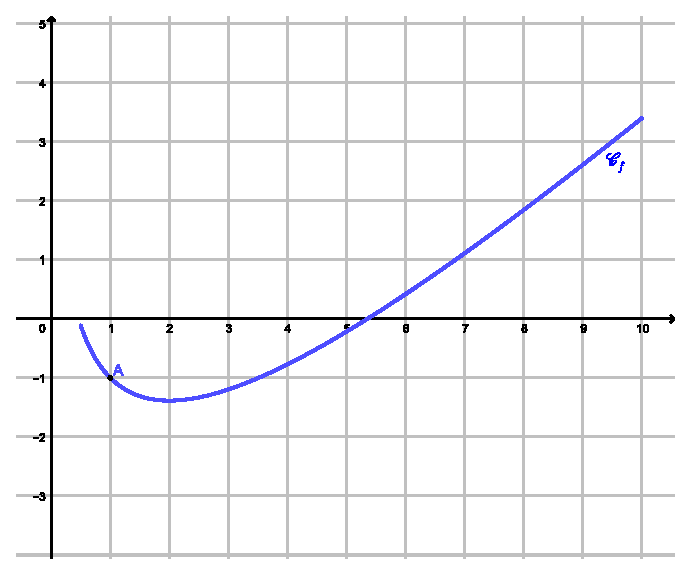
\includegraphics[width=0.7\textwidth]{images/BBESL-s4-3-1.eps}% gbb 1 unite=1cm
     \end{extern}
\end{center}

\begin{enumerate}
     \item %1
     Montrer que pour tout réel $x$ appartenant à l'intervalle $[0,5~;~10]$ :
     \[ f'(x) =\dfrac{x-2}{x}. \]
     \item %2
     Dresser le tableau de variations de $f$ sur l'intervalle $[0,5~;~10]$.
     \item %3
     Déterminer l'équation réduite de la tangente $T$ à la courbe $\mathscr{C}_f$ au point $A(1~;~-1)$.
     \item %4
     \'Etudiez la convexité de $f$ sur l'intervalle $[0,5~;~10]$.
     \item %5
     Montrer que l'équation $f(x)=0$ admet une et une seule solution $\alpha$ sur l'intervalle $[0,5~;~10]$.
     \par
     Donner un encadrement de $\alpha$ d'amplitude $10^{-2}$.
     \item %6
     Montrer que la fonction $F$ définie par :
     \[ F(x)=\dfrac{x^2}{2} - 2x\ln x \]
     est une primitive de la fonction $f$ sur l'intervalle $[0,5~;~10]$.
     \item %7
     Donner la valeur exacte, puis la valeur arrondie à $10^{-2}$, de l'intégrale :
     \[ I=\displaystyle\int_{6}^{10} f(t)dt. \]
     Interpréter graphiquement la valeur de cette intégrale.
     \par
\end{enumerate}
\begin{corrige}
     \begin{enumerate}
          \item %1
          Sur l'intervalle $[0,5~;~10]$, la fonction $f$ est dérivable comme somme de fonctions dérivables et :
          \par
          $f'(x)=1-2 \times \dfrac{1}{x}=\dfrac{x}{x}-\dfrac{2}{x}=\dfrac{x-2}{x}$.
          \par
          \cadre{rouge}{À retenir}{
               La fonction logarithme népérien est définie et dérivable sur l'intervalle $]0~;~+\infty[$ et a pour dérivée la fonction $x \longmapsto \dfrac{1}{x}$.
          }
          \item %2
          $x$ est strictement positif sur l'intervalle $[0,5~;~10]$ ; la fonction $f'$ est donc du signe de $x-2$, c'est à dire qu'elle s'annule pour $x=2$ et est strictement positive pour $x>2$.
          \par
          De plus :
          \par
          $f(2)=2-2-2\ln2=-2\ln2$ ;
          \par
          $f(0,5)=0,5-2-2\ln(0,5)=0,5-2-2\ln\left(\dfrac{1}{2}\right)=-1,5+2\ln2$ ;
          \par
          $f(2)=10-2-2\ln10=8-2\ln10$.
          \par
          On obtient le tableau de variations suivant :
          \par
          %:-+-+-+-+- Engendré par : http://math.et.info.free.fr/TikZ/TableauxVariations/
          \begin{center}
               \begin{extern}%width="400" alt="tableau de variation de la fonction f"
                    \begin{tikzpicture}[scale=0.875]
                         % Styles
                         \tikzstyle{cadre}=[thin]
                         \tikzstyle{fleche}=[->,>=latex,thin]
                         \tikzstyle{nondefini}=[lightgray]
                         % Dimensions Modifiables
                         \def\Lrg{1.5}
                         \def\HtX{1}
                         \def\HtY{0.5}
                         % Dimensions Calculées
                         \def\lignex{-0.5*\HtX}
                         \def\lignef{-1.5*\HtX}
                         \def\separateur{-0.5*\Lrg}
                         % Largeur du tableau
                         \def\gauche{-1.5*\Lrg}
                         \def\droite{5.5*\Lrg}
                         % Hauteur du tableau
                         \def\haut{0.5*\HtX}
                         \def\bas{-2.5*\HtX-2*\HtY}
                         % Ligne de l'abscisse : x
                         \node at (-1*\Lrg,0) {$x$};
                         \node at (0.5*\Lrg,0) {$0,5$};
                         \node at (2.5*\Lrg,0) {$2$};
                         \node at (4.5*\Lrg,0) {$10$};
                         % Ligne de la dérivée : f'(x)
                         \node at (-1*\Lrg,-1*\HtX) {$f'(x)$};
                         \node at (0.5*\Lrg,-1*\HtX) {$\ $};
                         \node at (1.5*\Lrg,-1*\HtX) {$-$};
                         \node at (2.5*\Lrg,-1*\HtX) {$0$};
                         \node at (3.5*\Lrg,-1*\HtX) {$+$};
                         \node at (4.5*\Lrg,-1*\HtX) {$$};
                         % Ligne de la fonction : f(x)
                         \node  at (-1*\Lrg,{-2*\HtX+(-1)*\HtY}) {$f(x)$};
                         \node (f1) at (0.5*\Lrg,{-2*\HtX+(0)*\HtY}) {$2\ln2-1,5$};
                         \node (f2) at (2.5*\Lrg,{-2*\HtX+(-2)*\HtY}) {$-2\ln2$};
                         \node (f3) at (4.5*\Lrg,{-2*\HtX+(0)*\HtY}) {$8-2\ln10$};
                         % Flèches
                         \draw[fleche] (f1) -- (f2);
                         \draw[fleche] (f2) -- (f3);
                         % Encadrement
                         \draw[cadre] (\separateur,\haut) -- (\separateur,\bas);
                         \draw[cadre] (\gauche,\haut) rectangle  (\droite,\bas);
                         \draw[cadre] (\gauche,\lignex) -- (\droite,\lignex);
                         \draw[cadre] (\gauche,\lignef) -- (\droite,\lignef);
                    \end{tikzpicture}
               \end{extern}
          \end{center}
          \item %3
          L'équation réduite de la tangente $T$ à la courbe $\mathscr{C}_f$ au point $A$ d'abscisse $1$ est :
          \par
          $y=f'(1)(x-1)+f(1).$
          \par
          Or :
          \par
          $f(1)=1-2-2\ln(1)=-1\ $ et $f'(1)=\dfrac{1-2}{1}=-1.$
          \par
          L'équation réduite de $T$ est donc :
          \par
          $y=-1(x-1)-1$
          \par
          $y=-x.$
          \par
          \textit{(N.B. : Cette droite passe par le point $A$ et par l'origine du repère.)}
          \par
          \cadre{rouge}{À retenir}{
               L'équation réduite de la tangente à la courbe représentative de $f$ au point d'\textbf{abscisse} $\bm{a}$ est :
               \[ y=f'(a)(x-a)+f(a). \]
          }
          \item %4
          La fonction $f'$ est dérivable sur l'intervalle $[0,5~;~10]$ ; posons :
          \par
          $u(x)=x-2\ $ et $\ v(x)=x.$
          \par
          Alors :
          \par
          $u'(x)=1\ $ et $\ v('x)=1$.
          \par
          Par conséquent :
          \par
          $f''(x)=\dfrac{u'(x)v(x)-u(x)v'(x)}{v(x)^2}$
          \par
          $\phantom{f''(x)}=\dfrac{x-(x-2)}{x^2}$
          \par
          $\phantom{f''(x)}=\dfrac{2}{x^2}$.
          \par
          $f''(x)$ est strictement positive  sur l'intervalle $[0,5~;~10]$ donc la fonction $f$ est \textbf{convexe} sur cet intervalle.
          \item %5
          $f(0)=2\ln2-1,5 \approx -0,11 < 0$ ;
          \par
          $f(2)=2\ln2 \approx -1,39 < 0$ ;
          \par
          $f(10)= 8-2\ln10 \approx 3,39 >0$.
          \par
          D'après le tableau de variations de la question \textbf{2.}, on voit que :
          \par
          \begin{itemize}
               \item
               Pour $x \in [0,5~;~2]$, $f(x)$ est strictement négatif (car inférieur à $f(0)$ qui est négatif).
               \par
               L'équation $f(x)=0$ n'a donc pas de solution sur cet intervalle.
               \item
               Sur l'intervalle $[2~;~10]$, $f$ est \textbf{continue}, \textbf{strictement croissante} et \textbf{change de signe} entre 2 et 10. Donc l'équation $f(x)=0$ admet une unique solution sur l'intervalle $[2~;~10]$.
               \par
               Par conséquent, l'équation $f(x)=0$ admet une unique solution sur l'intervalle $[0,5~;~10]$.
               \par
               \`A la calculatrice, on trouve :
               \par
               $f(5,35) \approx -0,004 < 0$ ;
               \par
               $f(5,36) \approx 20,002 > 0$.
               \par
               Par conséquent :
               \[ 5,35 < \alpha < 5,36. \]
          \end{itemize}
          \item %6
          Pour montrer que $F$ est une primitive de $f$  sur l'intervalle $[0,5~;~10]$, il suffit de montrer que $F'=f$.
          \par
          La dérivée de la fonction $x \longmapsto \dfrac{x^2}{2}$ est la fonction ${x \longmapsto \dfrac{2x}{2}=x}$.
          \par
          Pour calculer la dérivée de la fonction $x \longmapsto -2x\ln x$ on pose :
          \par
          $u(x)=-2x\ $ et $\ v(x)=\ln x$.
          \par
          Alors :
          \par
          $u'(x)=-2\ $ et $\ v('x)=\dfrac{1}{x}$ ;
          \par
          et :
          \par
          $u'(x)v(x)+u(x)v'(x)=-2\ln x - 2x \times \dfrac{1}{x}=-2\ln x - 2$.
          \par
          Par conséquent :
          \par
          $F'(x) = x -2\ln x - 2 = f(x)$.
          \par
          La fonction $F$ est donc une primitive de la fonction $f$ sur l'intervalle $[0,5~;~10]$.
          \par
          \cadre{vert}{En pratique}{
               Pour montrer qu'une fonction $F$ est une primitive de la fonction $f$ sur un intervalle $I$, on calcule la dérivée $F'$ de $F$ et on montre que $F'=f$.
          }
          \item %7
          La fonction $F$ étant une primitive de la fonction $f$ sur l'intervalle $[0,5~;~10]$, on a :
          \par
          $I=\displaystyle\int_{6}^{10}f(t)\text{d}t=\left[F(t)\right]_6^{10}=F(10)-F(6)$
          \par
          $\phantom{I}=\dfrac{10^2}{2} - 20\ln 10 - \left[\dfrac{6^2}{2} - 12\ln 6\right]$
          \par
          $\phantom{I}=50 - 20\ln 10 - 18 + 12\ln 6$
          \par
          $\phantom{I}=32 - 20\ln 10 + 12\ln 6$
          \par
          $I \approx 7,45$ (arrondi au centième).
          \par
          La fonction $f$ étant positive sur l'intervalle $[6~;~10]$, l'intégrale $I$ est égale à l'aire, exprimée en unités d'aire, du domaine délimité par la courbe $\mathscr{C}_f$, l'axe des abscisses et les droites d'équations respectives $x=6$ et $x=10$.
          \par
          \cadre{rouge}{À retenir}{
               Pour calculer l'intégrale $\displaystyle\int_{a}^{b}f(x)\text{d}x$ alors que l'on connaît une primitive $F$ de $f$ sur l'intervalle $[a~;~b]$, on utilise la formule :
               \[  \displaystyle\int_{a}^{b}f(x)\text{d}x = [F(x)]_a^b = F(b)-F(a). \]
               \par
          }
          \cadre{bleu}{Remarque}{
               La variable $x$ dans l'expression $\displaystyle\int_{a}^{b}f(x)\text{d}x$ est une variable \og muette \fg{}.
               \par
               Cela signifie qu'elle n'apparaît pas dans le résultat du calcul et que l'on peut lui substituer n'importe quelle autre lettre ; par exemple il est équivalent d'écrire $\displaystyle\int_{a}^{b}f(x)\text{d}x$ ou $\displaystyle\int_{a}^{b}f(t)\text{d}t$.
          }
     \end{enumerate}
\end{corrige}

\end{document}